\section{放射線試験(寺田(報告書)・池谷・黒崎)}
\subsection*{関連文書}
\begin{itemize}
	\item OP-S1-0126 球状太陽電池放射線試験結果
\end{itemize}
\subsection{試験概要}
\subsubsection{目的}
本試験では,多量の放射線が入射することに起因する電離効果のうち,トータルイオンドーズ効果が機器に与える恒久的損傷を調べた.これにより,新規開発基盤である通信\&インヒビット基板(CIB)および膜上デバイス制御(MDC)基板に関して,ミッション期間中に受ける損傷具合を試験した.

シングルイベント(Single Event Effects=SEE)試験はプロジェクトの進行状況および人員を考慮し行われなかったものの,本来は実施されるべきである.


表\ref{table_4_date}に全5回の試験日時,$\gamma$線照射時間をまとめた.
\begin{table}[htbp]
	\centering
	\caption{放射線試験 試験日時一覧}
	\label{table_4_date}
	\begin{tabular}{ccccc}
		\hline\hline
		回& 日付 & 開始 & 終了 & 最大照射時間[h]  \\ \hline
		1&2017/2/6 &11:00  &17:30&6.0  \\
		2&2017/7/13  &14:00  &18:00&3.0  \\
		3&2017/7/26  &11:00  &17:30&3.0  \\
		4&2018/2/9  &11:00  &16:30&3.0 \\
		5&2018/5/28  &14:00  &18:00&3.0 \\\hline\hline
	\end{tabular}
\end{table}

最初の放射線試験はBBM開発段階において,CIBやMDCの開発も進んでいない中,膜面搭載の球状太陽電池および膜面制御部に設置される赤外線LEDに関して,ミッション期間中に受ける損傷具合を試験した.続く第二回以降の試験ではCIB,MDC搭載のICを中心に試験が行われ,照射中にデータロガーを用いた電圧,電流,温度の計測が行われた.第三回以降ではさらにPCと通信させることにより,データ伝送が正常に行われるか確認した.第四回試験ではEM開発中に増えたIC並びに,照射量が不十分であったICの試験を行った.第四回で通信用のマイコンに不具合発生が確認されたた,最後に追試験(第五回)を行い搭載するマイコンを変更した.

\vspace{3ex} 
\textbf{コメント}
\begin{itemize}
\item 実験室を予約する場合は,照射時間だけでなく,前後の準備撤収時間を考慮し最低1時間は余分に予約する.
\item 第5回試験では1名のみで当日,準備から実験まで行ったが,照射室とPC等を置く場所は離れているので,2名いた方が準備しやすいと思う.
\item 上記コメントに追記:照射中は最大二人,セットアップと撤収には最低二人必要であると考える.
\end{itemize}
	
\subsubsection{試験場所}
東京工業大学 大岡山キャンパス 大岡山北実験棟1 コバルト60照射室

\vspace{3ex} 
\textbf{コメント}
\begin{itemize}
	\item 予約はメールでやり取りを行う.
\end{itemize}


\subsection{試験供試体および照射条件}

供試体一覧を表\ref{tab:tidic}に示す.


\begin{landscape}
\begin{table}[htbp]
	\centering
	\caption{放射線試験 試験供試体,照射量,試験条件,および確認項目}
	\label{tab:tidic}
	
	%\scalebox{0.9}{
	\scriptsize
	\begin{tabular}{c|c|c|c|c|c|c|c|l|l}
		\hline\hline
		回                   &                      & 型番                   & 搭載箇所                 & 線量       & 照射時間         & 距離           & データロガー計測項目           & その他確認項目                 & 備考                    \\
		                   &                      &                  &                 & {[}Gy{]}        &  {[}h{]}         & {[}cm{]}          &           &                &                  \\ \hline
		1   & 球状太陽電池               &                      & 膜                    & 14883                & 6                    & 10                   &                      & 点灯確認                 &                       \\
		& 赤外線LED               & OSI5LA5113A          & 膜展開部                 & 14883                & 6                    & 10                   &                      & 点灯確認                 &                       \\\hline
		2   & DCDCコンバータ            & TPS55330             & CIB                  & 39                   & 0.5                  & 60                   & 出力電圧,入力電流,温度         &         &                       \\
		& リニアレギュレータ            & TA78033AF         & CIB                  & 39                   & 0.5                  & 60                   & 出力電圧,入力電流,温度         &         &                       \\
		& ダイオード                & B540-13-F            & CIB                  & 39                   & 0.5                  & 60                   &                      & 逆電流が流れないか            &                       \\
		& オペアンプ                & AD8657ARM            & MDC                  & 39                   & 0.5                  & 60                   & 温度                   & 照射前後の機能確認         &                       \\\hline
		3  & マイコン                 & PIC16F887            & CIB                  & 231                  & 3                    & 60                   & 入力電流                 &                      &                       \\
		& マイコン                 & PIC18F25K80          & MDC                  & 231                  & 3                    & 60                   & 入力電流                 &                      &                       \\
		& CANトランシーバ            & MAX3051ESA+          & MDC                  & 231                  & 3                    & 60                   & 入力電流                 & mbedにより信号確認          & 80分(103 Gy分)後動作不良 \\
		& シャントレギュレータ           & TL431                & MDC                  & 231                  & 3                    & 60                   & 出力電圧,入力電流,温度         & 出力電圧,入力電流,温度         &                       \\
		& 加速度センサ               & ADXL345              & CIB                  & 231                  & 3                    & 60                   & 入力電流                 &                      &                       \\
		& ジャイロセンサ              & ITG-3200             & CIB                  & 231                  & 3                    & 60                   & 入力電流                 &                      &                       \\
		& 対数検出器                & ADL5513ACPZ          & 膜上アンテナ               & 16830                & 3                    & 0                    & 出力電圧,入力電流            &                      &                       \\\hline
		4  & マイコン                 & PIC16F887            & CIB                  & 213                  & 3                    & 60                   &                      & mbedにより信号確認          & 60分(71 Gy分)後動作不良  \\
		& マイコン                 & PIC16F886            & CIB                  & 213                  & 3                    & 60                   &                      & mbedにより信号確認          &                       \\
		& DCDCコンバータ            & TPS55330             & CIB                  & 213                  & 3                    & 60                   & 出力電圧                 &                      &                       \\
		& モデム                  & FX614                & CIB                  & 213                  & 3                    & 60                   &                      & mbedにより信号確認          &                       \\
		& ADコンバータ              & MAX11605             & CIB                  & 213                  & 3                    & 60                   &                      & mbedにより信号確認          &                       \\
		& ダイオード                & B540-13-F            & CIB                  & 213                  & 3                    & 60                   &                      & mbedにより電圧確認          &                       \\
		& レギュレータ               & TA78033AF            & CIB                  & 213                  & 3                    & 60                   &                      & mbedにより電圧確認          &                       \\
		& MOSFET               & SK8603140L           &                      & 213                  & 3                    & 60                   & 出力電圧                 &                      & 搭載されず                 \\
		& ダイオード                & RB080L-30            & CIB                  & 213                  & 3                    & 60                   &                      & mbedにより電圧確認          &                       \\
		& PhotoMOS             & AQY211G2S            & CIB                  & 213                  & 3                    & 60                   & 出力電圧                 &                      &                       \\
		& PhotoMOS             & AQV252G3S            & CIB, MDC             & 213                  & 3                    & 60                   & 出力電圧                 &                      &                       \\
		& タイマー                 & SA555                &                      & 213                  & 3                    & 60                   & 出力電圧                 &                      &                       \\
		& マルチプレクサ              & ADG821BRMZ           &                      & 213                  & 3                    & 60                   & 出力電圧                 &                      &                       \\
		& レギュレータ               & TA7805AF             &                      & 213                  & 3                    & 60                   &                      & mbedにより電圧確認          & 搭載されず                 \\
		& MOSFET               & MTM232230LBF         &                      & 213                  & 3                    & 60                   & 出力電圧                 &                      &                       \\
		& マイコン                 & PIC18F25K80          & MDC                  & 71                   & 1                    & 60                   &                      & 照射前後の機能確認            &                       \\
		& CANトランシーバ            & MAX3051ESA+          & MDC                  & 71                   & 1                    & 60                   &                      & mbedにより信号確認          &                       \\
		& 加速度センサ               & ADXL345              & MDC                  & 71                   & 1                    & 60                   &                      & 照射前後の機能確認             &                       \\\hline
		5   & マイコン                 & PIC16F887            & CIB                  & 80                   & 3                    & 100                  &                      & mbedにより信号確認          &                       \\
		& マイコン                 & PIC16F886            & CIB                  & 80                   & 3                    & 100                  &                      & mbedにより信号確認          &                       \\
		& マイコン                 & PIC16F887            & CIB                  & 80                   & 3                    & 100                  &                      & mbedにより信号確認          &                       \\
		& WDT                  & SA555                & CIB                  & 80                   & 3                    & 100                  & 出力電圧                 &                      &  \\ \hline\hline
	\end{tabular}
\end{table}
\end{landscape}

図\ref{fig4-1-2}並びに,図\ref{fig4-1-4}はそれぞれ第四回,五回の供試体である.

\begin{figure}[htbp]
	\centering
	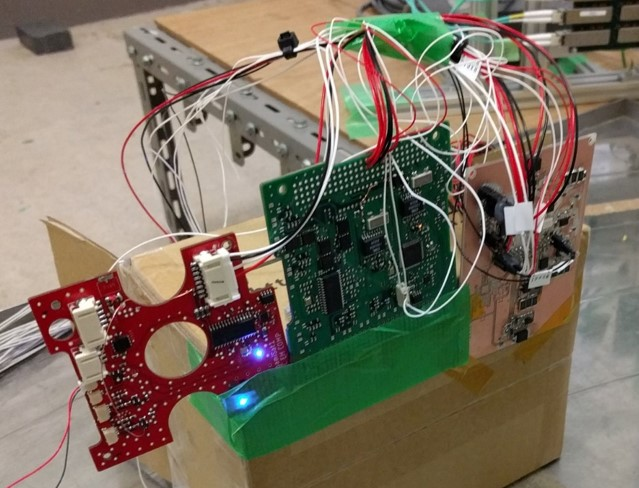
\includegraphics[scale=0.9]{04/fig/4-1-2.jpg}
	\caption{第四回試験供試体拡大図}
	\label{fig4-1-2}
\end{figure}

\begin{figure}[htbp]
	\centering
	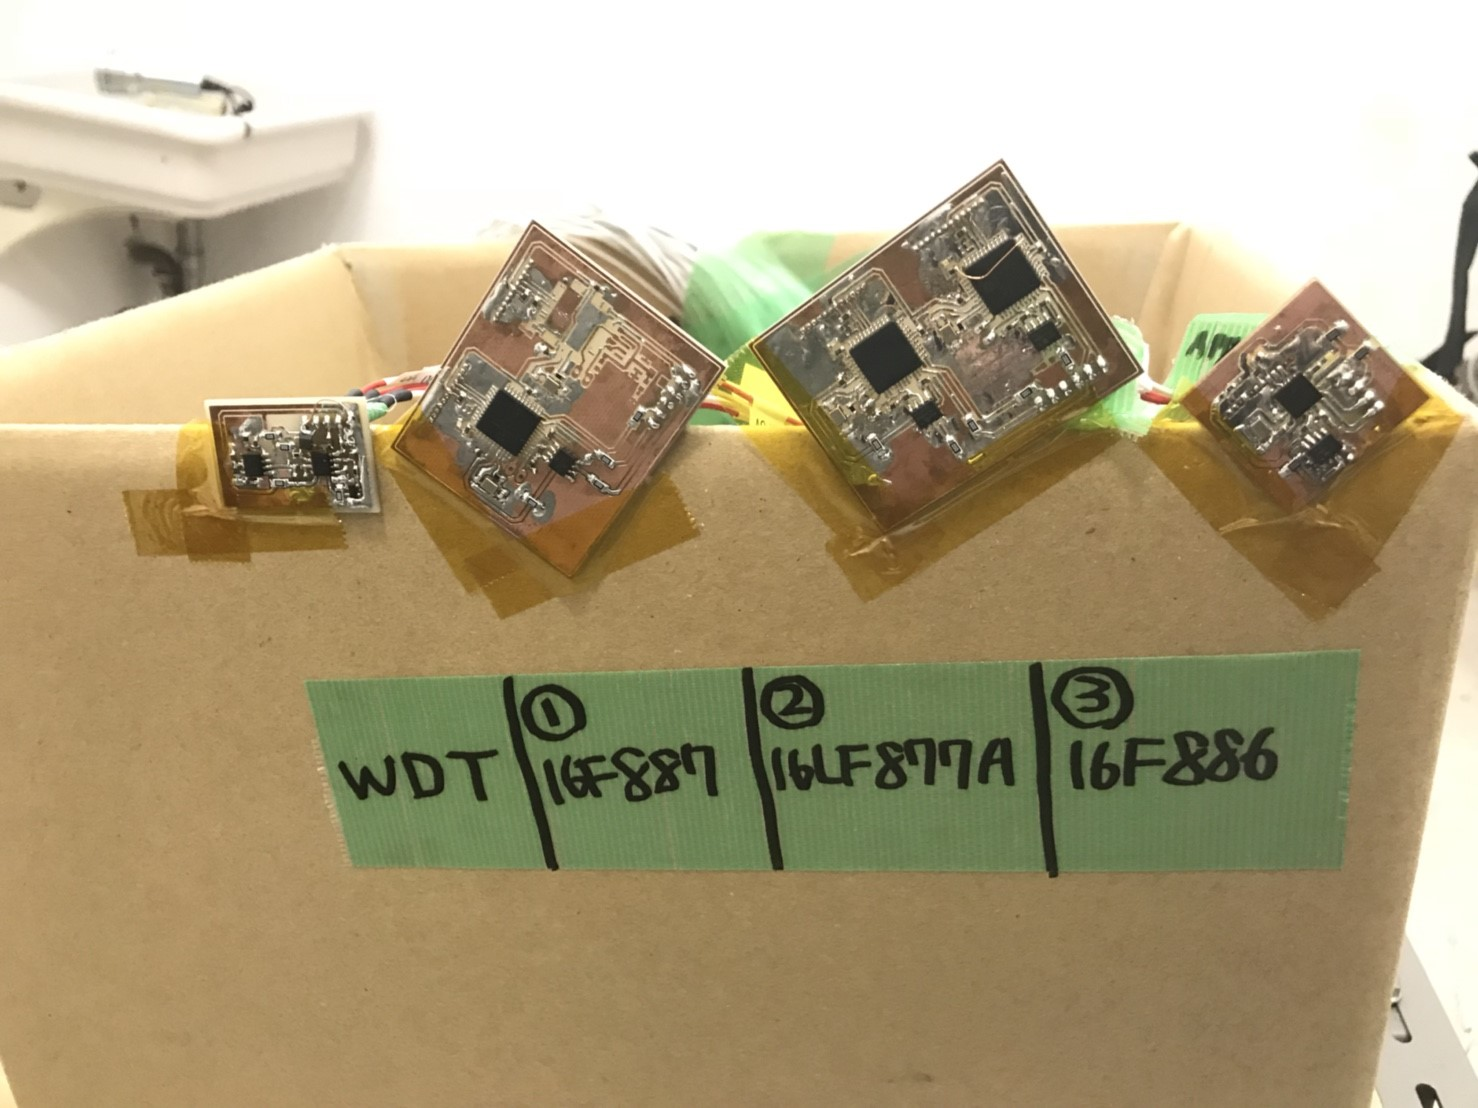
\includegraphics[width=70mm]{04/fig/4-1-4.jpg}
	\caption{第五回試験供試体拡大図}
	\label{fig4-1-4}
\end{figure}


\vspace{2ex} 
\textbf{コメント}
\begin{itemize}
	\item 第五回試験を第四回と異なる試験条件(線源までの距離,照射時間)で試験を行ったが,第四回と試験条件を揃えるべきだったかもしれない.
\end{itemize}



\subsection{照射量}
OrigamiSat-1のCIB周り,およびMDC基板周りのアルミニウム構体板厚は2 mmである.NASA SSP 30512 Revision C によると高度500km,軌道系射角 $51.6 ^{\circ}$の環境において厚さ2.032 mmのアルミニウムに囲まれている場合の1年あたりトータルドーズ量 1.012E+03 rad(10.12 Gy)である.使用期間をCI基板は1年,MDC基板は4か月とした場合の被ばく量はそれぞれ約10.12 Gy,3.73 Gyとなる.第四回試験においては,両基板ともに両面にICが搭載されているため0.5 hごとに基板の表裏をひっくり返した.線源に対して裏面にあるICの被ばく量は表面にあるICの被ばく量に対して微小であると仮定した.

参考としてコバルト60照射室の線量率と線源からの距離の関係を表\ref{tab:tidrate}にまとめた.
さらに線源から60 cm,100 cmの距離に置かれた実験の様子を図\ref{fig4-1-1},図\ref{fig4-1-3}に示す.

\begin{table}[htbp]
	\centering
	\caption{コバルト60照射室 線量率}
	\label{tab:tidrate}
	
	\begin{tabular}{c|cccc}
		\hline\hline
		距離(cm)   & 0        & 10       & 60       & 100      \\
		単位(Gy/h) & $\times10^3$     & $\times10^3$     & $\times10^2$        & $\times10$      \\ \hline
		2017.2   & 5.926781 & 2.590717 & 0.814838 & 3.147849 \\
		2017.7        & 5.610307 & 2.45238  & 0.771328 & 2.979763 \\
		2018.2   & 5.195429 & 2.271029 & 0.714289 & 2.759412 \\
		2018.5        & 5.027153 & 2.197471 & 0.691154 & 2.670036 \\ \hline\hline
	\end{tabular}
\end{table}



\begin{figure}[htbp]
	\centering
	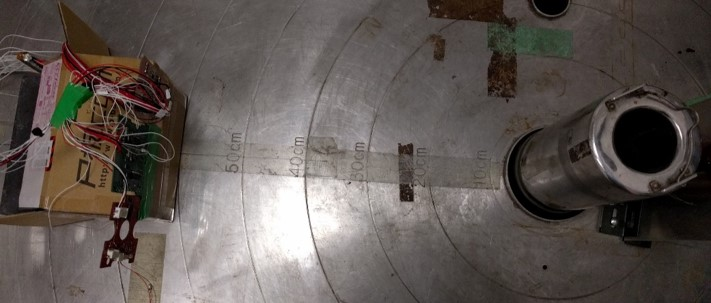
\includegraphics[scale=0.9]{04/fig/4-1-1.jpg}
	\caption{第四回配置の様子}
	\label{fig4-1-1}
\end{figure}


\begin{figure}[htbp]
	\centering
	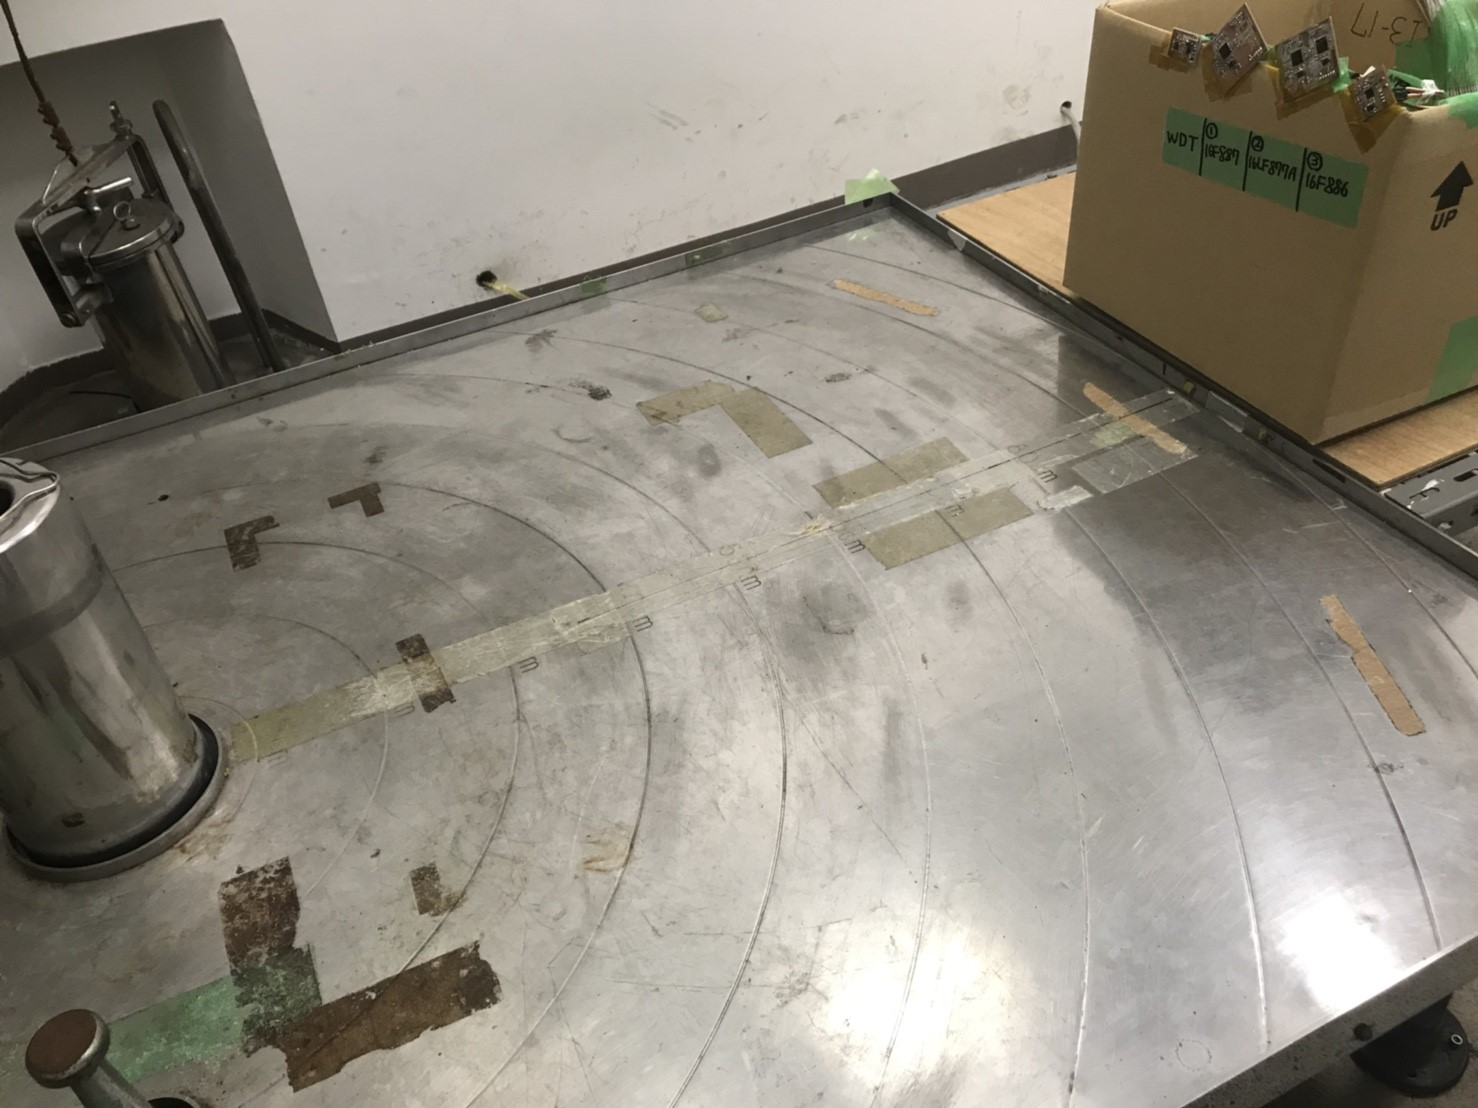
\includegraphics[width=70mm]{04/fig/4-1-3.jpg}
	\caption{第五回配置の様子}
	\label{fig4-1-3}
\end{figure}

\subsection{検証方法}
図\ref{fig4-1-0}の通りに,デバイスを配置し,データロガー及びPCでデータをモニタリングした.
ターミナルブロックは試験室内外を結ぶDsub 50ピンのコネクタに接続された.
$\textrm{I}^2 \textrm{C}$通信やSPI通信は長距離通信に不向きであるため,試験室内にmbed NXP LPC1768を鉛で保護しつつ配置しmbedからUARTによって試験室内外で通信した.

\begin{figure}[H]
	\centering
	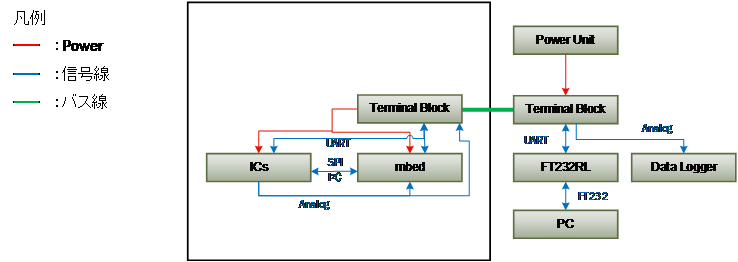
\includegraphics[width=150mm]{04/fig/4-1-0.png}
	\caption{試験セットアップ概要図.長方形内が放射線試験室を示している.}
	\label{fig4-1-0}
\end{figure}
\begin{figure}[H]
	\centering
	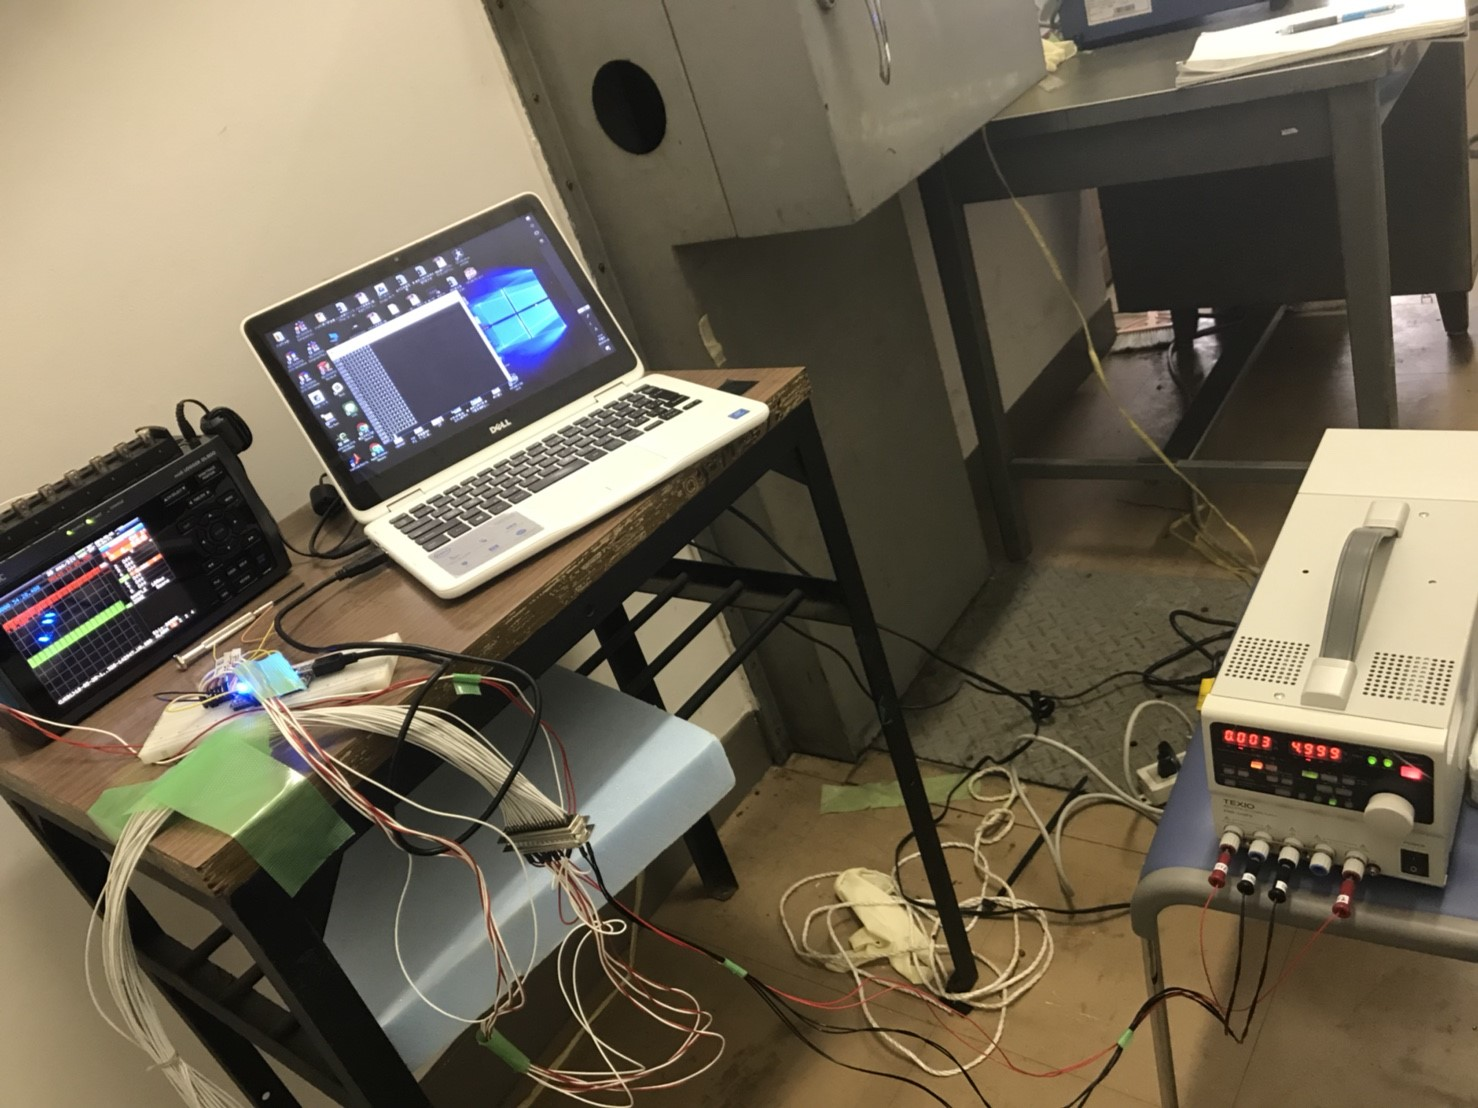
\includegraphics[width=70mm]{04/fig/4-1-5.jpg}
	\caption{照射室外の様子.データロガー,外部電源,PCなどがある.}
	\label{fig4-1-5}
\end{figure}

\vspace{2ex} 
\textbf{コメント}
\begin{itemize}
	\item 放射線照射室とPC等を置くう照射室外を繋ぐ図\ref{fig4-1-0}の緑ハーネス部分は,コバルト60照射室の設備としてDサブハーネスが既にある.ただ,Dサブハーネスと接続するケーブルは両側,事前に作成しておく必要がある.事前にコバルト60照射室を見学しておくと,どのようなハーネスを作成しなければならないかイメージがつきやすいと思う.
	\item ハーネス作成時には,グラウンドを全て共有することを忘れずに.
\end{itemize}

\subsection{試験手順}
\begin{itemize}
	\item[ 1. ] 各コンポーネントを接続する
	\item[ 2. ]  順番に電源を投入する
	\item[ 3. ]  照射前に各ICが適切に動作していることを確認する
	\item[ 4. ]  照射:照射中はログを取る
	\item[ 5. ]  撤収する
	\item[ 6. ]  データの解析を行う
\end{itemize}

\vspace{2ex} 
\textbf{コメント}
\begin{itemize}
	\item 試験前日までに,放射線を照射しない状態で予定試験時間分ICが動作することを確認しておく.
\end{itemize}

\subsection{試験結果}

試験の結果,CANトランシーバー  MAX3051ESA+,およびにマイコン PIC16F887 の動作不具合が検出された.どちらのICもPCのターミナルソフト上での出力が,本来出力すべき文字から大きく逸脱し文字化けを起こした.

\begin{itemize}
	\item CANトランシーバー MAX3051ESA+ の不具合
	\item[ 症状:] 第三回試験において MAX3051ESA+ が103 Gy照射後動作不良を引き起こした.
	\item[ 原因:] CAN通信に不具合が発生したことが原因と思われる.
	\item[ 対策:] ミッション機器であり,さらに安全率を考慮して,ICを変更せず設計を進めた.
\end{itemize}

\begin{itemize}
	\item マイコン PIC16F887 の不具合
	\item[ 症状:] 第四回試験において PIC16F887 が71 Gy照射後動作不良を引き起こした.
	\item[ 原因:] UART通信もしくは$\textrm{I}^2 \textrm{C}$通信に不具合が発生したことが原因と思われる.
	\item[ 対策:] 地上局との通信用の非常に重要なICのため,宇宙利用実績のある PIC 16LF877A へと変更された.
\end{itemize}
